\chapter{Binärer Suchbaum}\label{ch:binarytree}

\section*{Lösung}

Gesucht ist der Baum, der folgendes Kriterium erfüllt\footnote{im Skript (Teil 2) auf Seite 143 in Defintion 6.3.3.1}:

\blockquote[{\cite[263, Hervorhebungen i.O.]{OW17e}}]{
    Für jeden Knoten \textit{p} gilt:
    Die Schlüssel im linken Teilbaum von \textit{p} sind sämtlich kleiner als der Schlüssel von \textit{p},
    und dieser ist wiederum kleiner als sämtliche Schlüssel im rechten Teilbaum von \textit{p}.
}

Da von den drei gegebenen Möglichkeiten nur eine Antwort richtig ist, können zwei Darstellungen ausgeschlossen werden.
Das gilt zum einen für den Baum, dessen Knoten\footnote{
    im Folgenden wird ``Noten mit dem Schlüssel \textit{[ZAHL]}`` zu ``Knoten \textit{[ZAHL]}`` abgekürzt
}~\textit{60} die~\textit{45} als direkten Nachfolger hat.
Diese Schlüssel gehören zu dem rechten Teilbaum des Knotens~\textit{50}, folglich ist das Kriterium, sämtliche Schlüssel im
\textit{rechten Teilbaum} müssen größer als~\textit{50} sein, verletzt, denn $45 < 50$.

Genauso ist der Baum, der den Knoten~\textit{60} mit direktem Nachfolger~\textit{85} enthält, kein den Kriterien entsprechender Suchbaum:
Da dieser Teilbaum der linke Teilbaum des Knotens~\textit{70} ist, muss für jeden Schlüssel innerhalb dieses Teilbaums gelten,
dass er kleiner als~\textit{70} ist, aber $85 > 70$).
\\

Der gesuchte Baum lässt sich folgendermaßen durch sukzessizes Einfügen der Schlüssel konstruieren:


\begin{figure}[h]
    \centering
    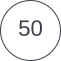
\includegraphics[
        width=1cm,
        keepaspectratio,
    ]{chapters/1. Binärer Suchbaum/img/50}
    \caption{Einfügen des Schlüssels 50.}

    \vspace{64}
\end{figure}

\begin{figure}[h]
    \centering
    \includegraphics[
        width=2cm,
        keepaspectratio,
    ]{chapters/1. Binärer Suchbaum/img/50 70}
    \caption{Einfügen der Schlüssel 50, 70.}

    \vspace{64}
\end{figure}

    \begin{figure}[h]
        \centering
    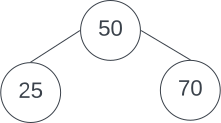
\includegraphics[
        width=3cm,
        keepaspectratio,
    ]{chapters/1. Binärer Suchbaum/img/50 70 25}
    \caption{Einfügen der Schlüssel 50, 70, 25.}
        \vspace{64}
\end{figure}


\begin{figure}[h]
    \centering
    \includegraphics[
        width=5cm,
        keepaspectratio,
    ]{chapters/1. Binärer Suchbaum/img/50 70 25 60}
    \caption{Einfügen der Schlüssel 50, 70, 25, 60.}

    \vspace{64}
\end{figure}

    \begin{figure}[h]
        \centering
    \includegraphics[
        width=5cm,
        keepaspectratio,
    ]{chapters/1. Binärer Suchbaum/img/50 70 25 60 45}
    \caption{Einfügen der Schlüssel 50, 70, 25, 60, 45.}

    \vspace{64}
    \end{figure}

        \begin{figure}[h]
            \centering
    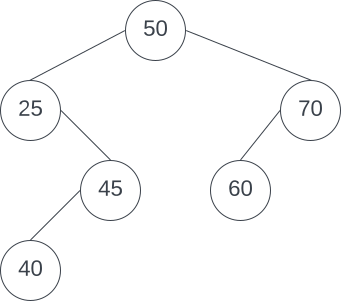
\includegraphics[
        width=6cm,
        keepaspectratio,
    ]{chapters/1. Binärer Suchbaum/img/50 70 25 60 45 40}
    \caption{Einfügen der Schlüssel 50, 70, 25, 60, 45, 40.}
            \vspace{64}
\end{figure}

\begin{figure}[h]
    \centering
    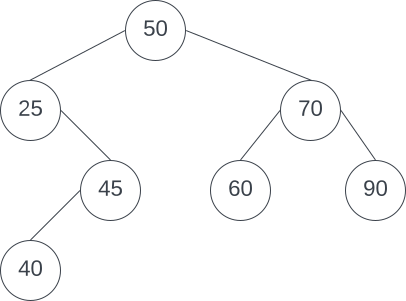
\includegraphics[
        width=7cm,
        keepaspectratio,
    ]{chapters/1. Binärer Suchbaum/img/50 70 25 60 45 40 90}
    \caption{Einfügen der Schlüssel 50, 70, 25, 60, 45, 40, 90.}

    \vspace{64}
\end{figure}

    \begin{figure}[h]
        \centering
    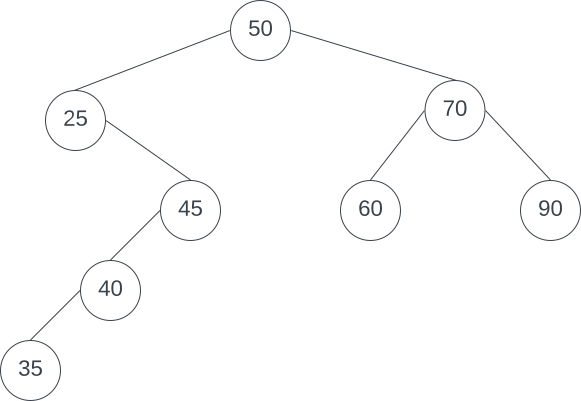
\includegraphics[
        width=9cm,
        keepaspectratio,
    ]{chapters/1. Binärer Suchbaum/img/50 70 25 60 45 40 90 35}
    \caption{Einfügen der Schlüssel 50, 70, 25, 60, 45, 40, 90, 35.}

    \vspace{64}
    \end{figure}

        \begin{figure}[h]
            \centering
    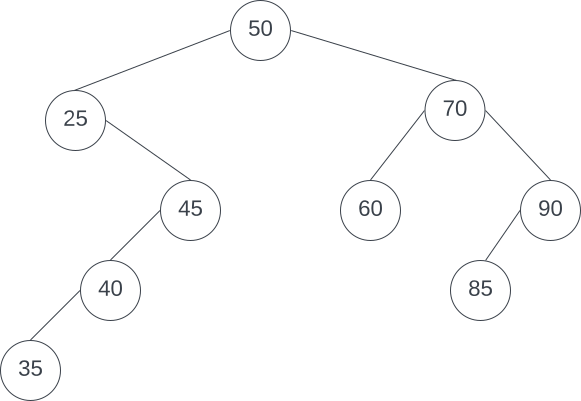
\includegraphics[
        width=9cm,
        keepaspectratio,
    ]{chapters/1. Binärer Suchbaum/img/50 70 25 60 45 40 90 35 85}
    \caption{Einfügen der Schlüssel 50, 70, 25, 60, 45, 40, 90, 35, 85.}
            \vspace{64}
\end{figure}

\begin{figure}[h]
    \centering
    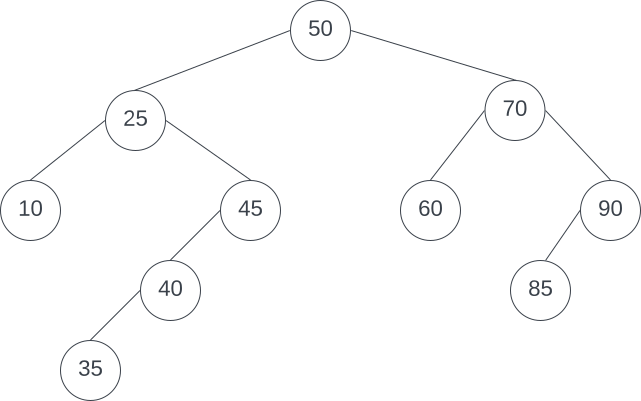
\includegraphics[
        width=9cm,
        keepaspectratio,
    ]{chapters/1. Binärer Suchbaum/img/50 70 25 60 45 40 90 35 85 10}
    \caption{Einfügen der Schlüssel 50, 70, 25, 60, 45, 40, 90, 35, 85, 10.}
\end{figure}